\subsection{Resumen}

El uso de la cache es el mismo sin importar el compilador: Usando programas para ver el contenido y el uso del cache (como por ejemplo valgrind) procesaremos varias imágenes, de distintos tamaños, e imágenes no cuadradas, para corroborar que sin importar el compilador, el uso de la cache es el mismo. \\


\subsection{Experimentaciones:}

Veremos a continuacion si el uso de la cache por ambos compiladores es similar, para esto relizaremos varias pasadas con los filtros implementados en c a diferentes imagenes. Esperamos ver que el funcionamiento de la cache es igual en ambos. \\

Para corroborar esto utilizaremos el valgrind, el cual nos muestra los misses y las  prediciones de saltos fallidas, dependiendo de esos resultados podremos concluir si el uso de la cache es igual de eficiente o si varia . \\

Primero veremos como es el comportamiento con el filtro blur, por cuestines de cuanto se tarda en emular la cache a medida que se aumenta el radio, decidimos probar los casos con un radio chico e ir aumentando solo el tamaño de la imagen. Si hay diferencias en el uso de la cache con radios chicos, con radios mas grandes esta diferencia se va a mantener o incluso aumentor, por eso consideramos que fijar el radio no perjudica nuestro experimento. \\

\subsection{Datos obtenidos:}

\begin{figure}[H]
\begin{center}
%\minipage{0.8\textwidth}
  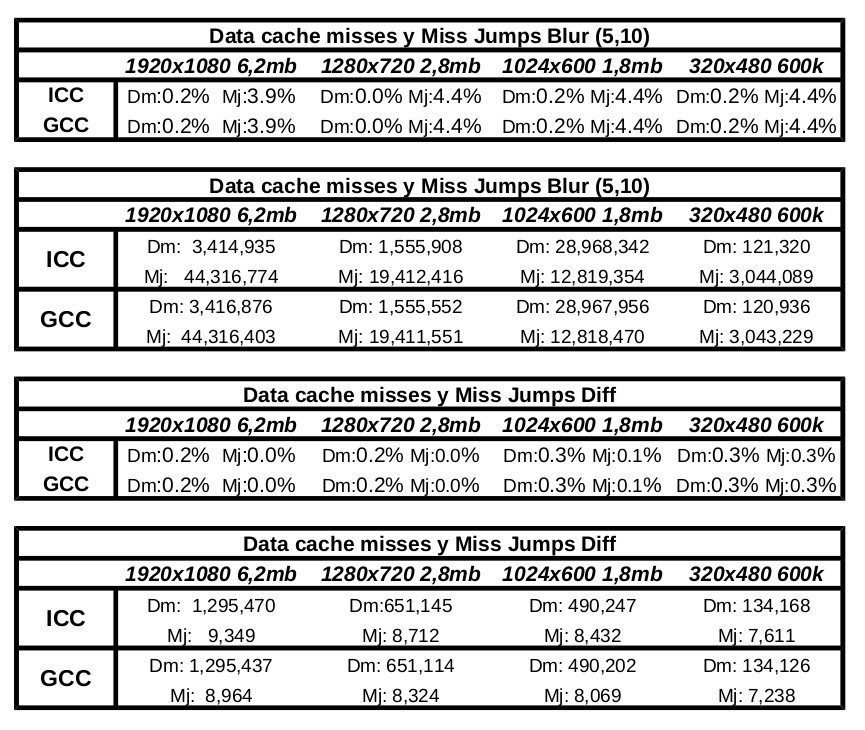
\includegraphics[width=\linewidth]{cachecompiladores/tabla.png}
%\endminipage
\end{center}
\end{figure}

\subsection{Conclusion:}

Luego de obtener los resultados y analizarlos observamos que si bien los valores de misses y miss jumps son muy parecidos , no son lo suficientemente parecidos como para concluir que el uso de la cache que hacen es el mismo. Esto lo deducimos de correr dos veces el mismo filtro a la misma imagen con un compilador, al ver los resultados varian en  casi nada (mas menos diez), pero si compramos los resultados de compiladores diferentes estas variaciones son suficientemente grandes como para ver que hacen usan la cache de formas diferentes. Por otro lado si miramos los porcentajes ambos tienen exatamente los mismos, por eso concluimos que no eran necesarios graficos, pues los valores son exactamente iguales, para cualquiera de los dos filtros, en cualquier situacion. Por ende concluimos que en realidad los compiladores manejan la cache de maneras distintas. Como un detalle, se puede ver que ICC tiende a tener mas misses y miss jumps que GCC. Antes habiamos visto que ICC es un poco mas rapido que GCC, bueno aqui podemos confirmar que eso no se debe a un mejor uso de la cache